% !TeX root = ../../main.tex
\section{Model implementation}

COMSOL was selected for detailed reactor modelling

\subsection{Model equations}




\subsection{Final results}
See \cref{fig:comsol-performance}.

\begin{figure}[h]
    \centering

    \begin{subfigure}{0.49\linewidth}
        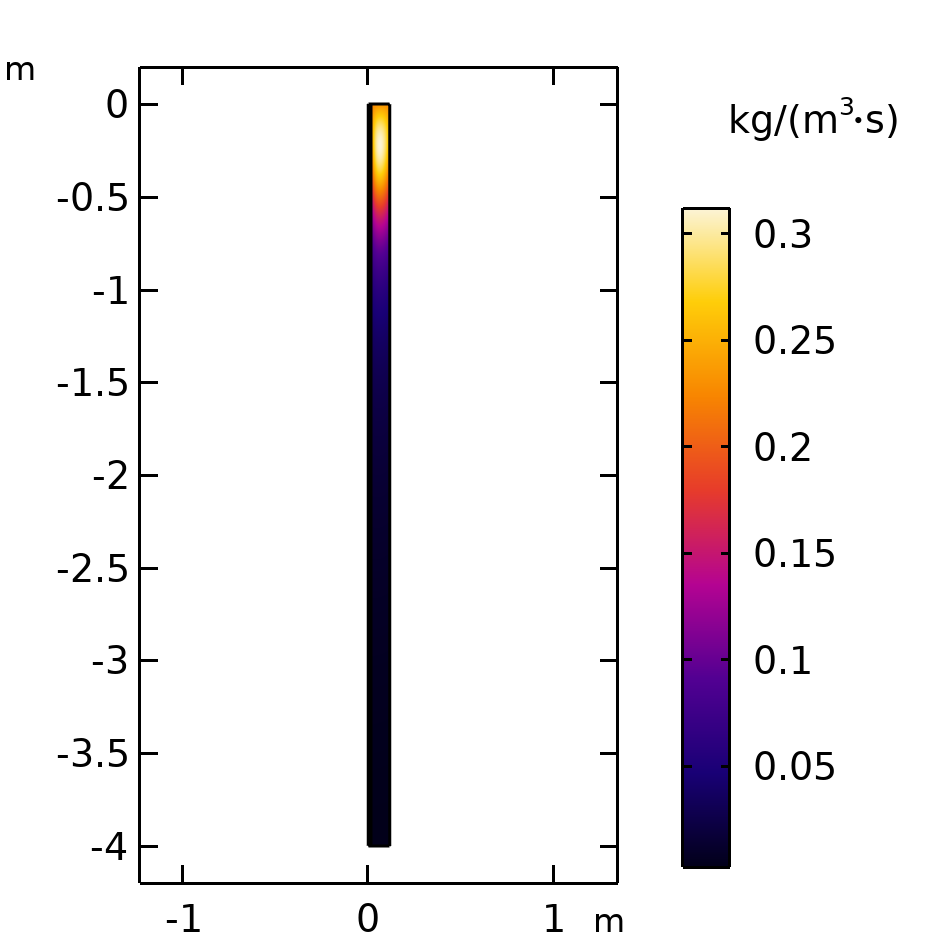
\includegraphics[width=\linewidth]{figures/r_TOL.png}
        \caption{Rate of Toluene reaction}
        \label{fig:comsol-performance:r_TOL}
    \end{subfigure}
    \begin{subfigure}{0.49\linewidth}
        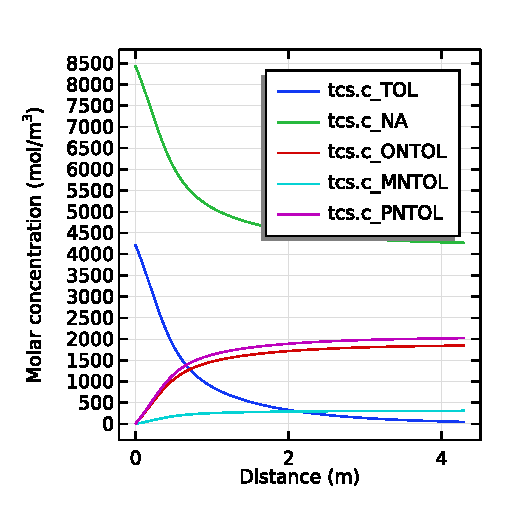
\includegraphics[width=\linewidth]{figures/concentration.eps}
        \caption{Concentration profile within reactor}
        \label{fig:comsol-performance:concentration}
    \end{subfigure}

    \caption{Reactor performance}
    \label{fig:comsol-performance}
\end{figure}

\subsubsection{Conversion}

See \cref{fig:comsol-conversion}.

\begin{figure}[h]
    \centering

    \begin{subfigure}{0.49\linewidth}
        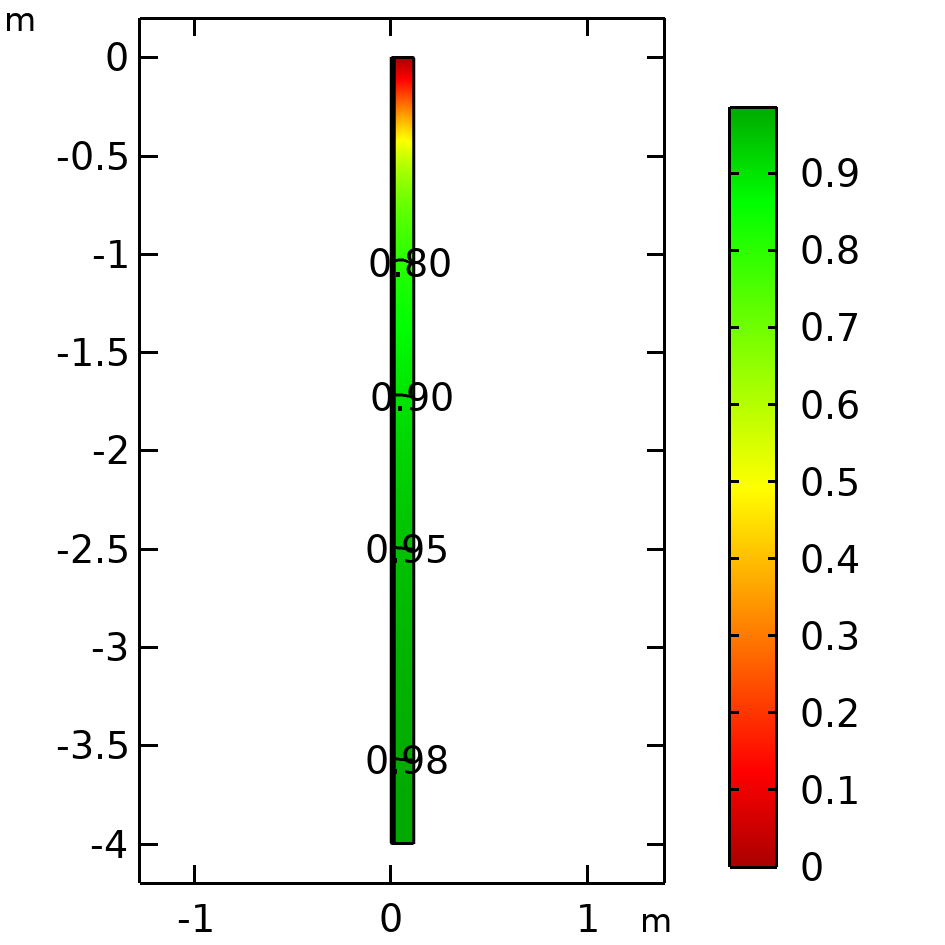
\includegraphics[width=\linewidth]{figures/conversion-surface.png}
        \caption{}
        \label{fig:comsol-conversion:surface}
    \end{subfigure}
    \begin{subfigure}{0.49\linewidth}
        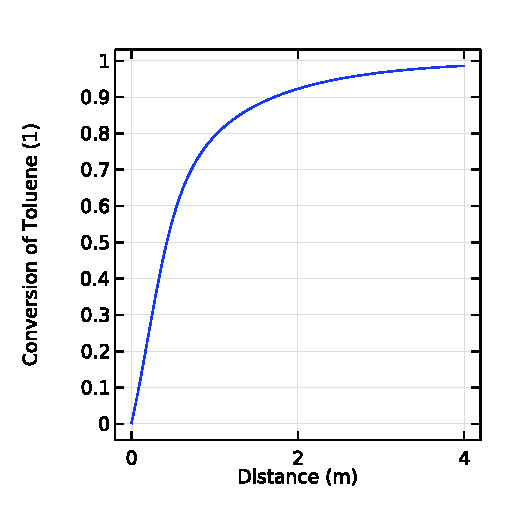
\includegraphics[width=\linewidth]{figures/conversion-line.eps}
        \caption{}
        \label{fig:comsol-conversion:line}
    \end{subfigure}

    \caption{Conversions}
    \label{fig:comsol-conversion}
\end{figure}

\subsubsection{Temperature}

See \cref{fig:comsol-temperature}.

\begin{figure}[h]
    \centering

    \begin{subfigure}{0.49\linewidth}
        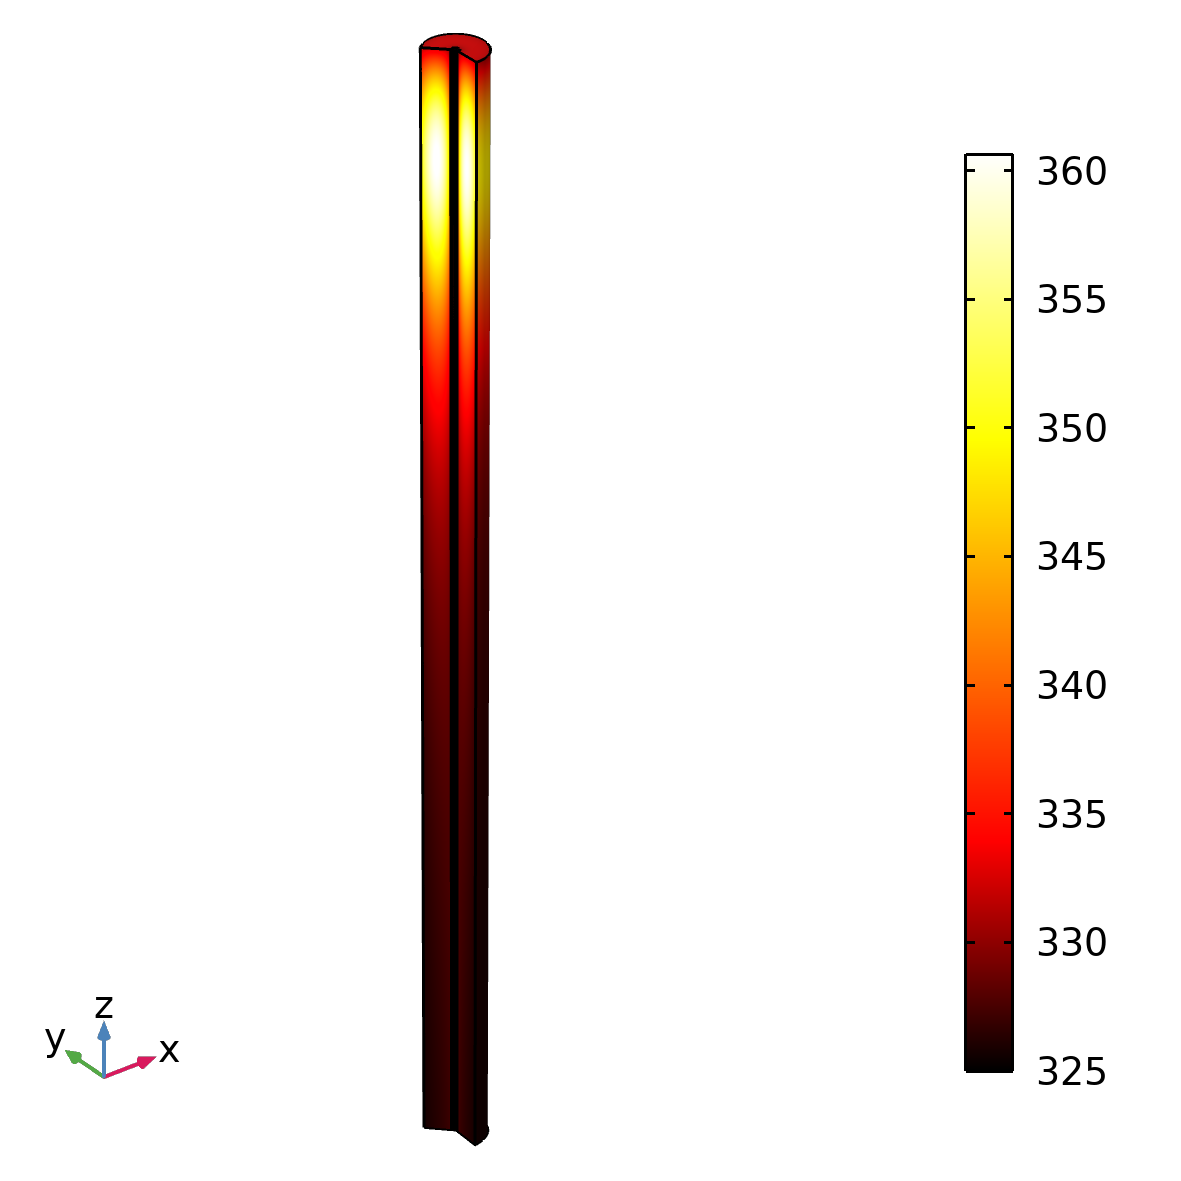
\includegraphics[width=\linewidth]{figures/temperature-surface.png}
        \caption{}
        \label{fig:comsol-temperature:surface}
    \end{subfigure}
    \begin{subfigure}{0.49\linewidth}
        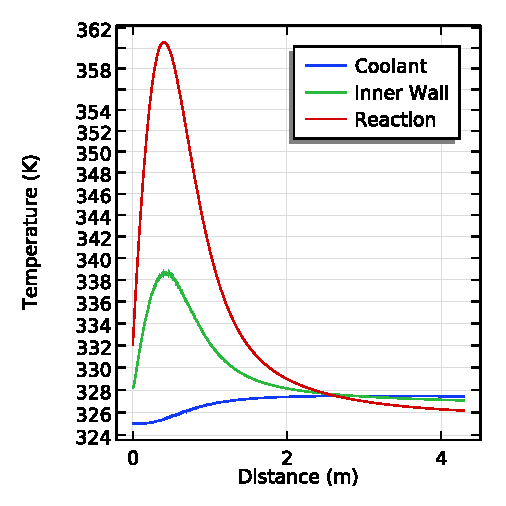
\includegraphics[width=\linewidth]{figures/temperature-lines.eps}
        \caption{}
        \label{fig:comsol-temperature:lines}
    \end{subfigure}

    \caption{Temperatures}
    \label{fig:comsol-temperature}
\end{figure}

\subsection{Optimisation and sensitivity analysis}

\subsubsection{Secondary cooling system sizing}

\begin{figure}[h]
    \centering

    \begin{subfigure}{0.49\linewidth}
        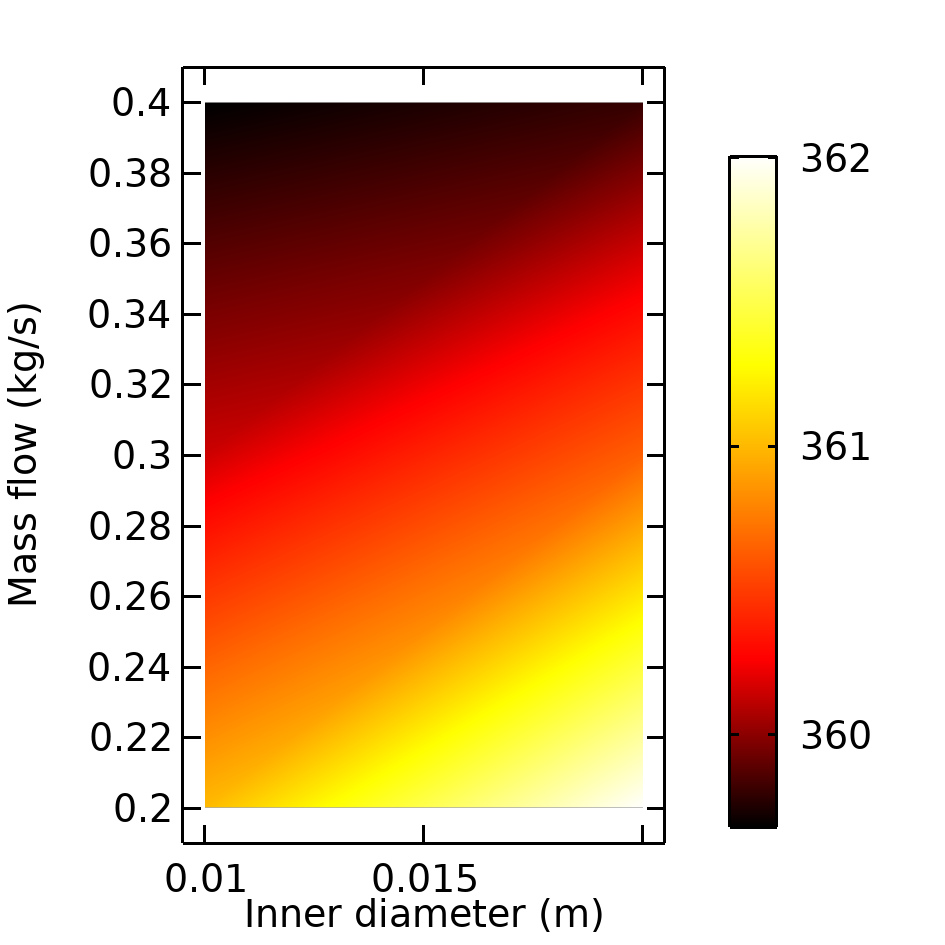
\includegraphics[width=\linewidth]{figures/S2-maxT.png}
        \caption{Maximum temperature reached in the reactor}
        \label{fig:comsol-S2:maxT}
    \end{subfigure}
    \begin{subfigure}{0.49\linewidth}
        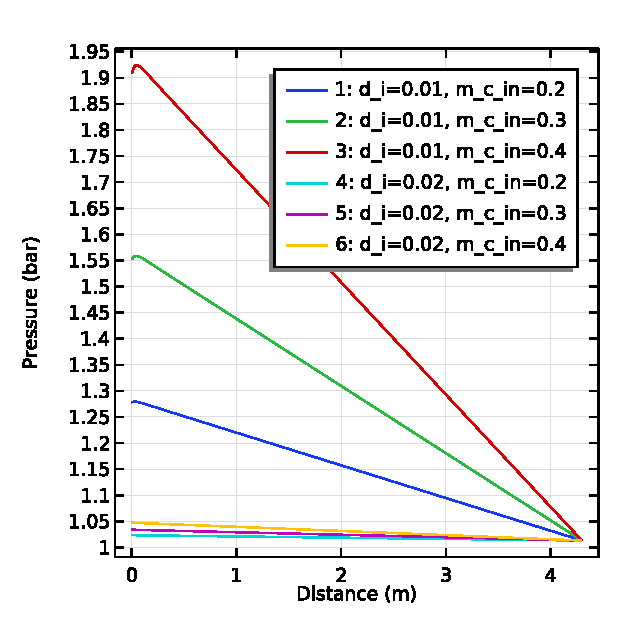
\includegraphics[width=\linewidth]{figures/S2-CW-Pdrop.eps}
        \caption{CW side pressure drop}
        \label{fig:comsol-S2:CW-Pdrop}
    \end{subfigure}

    \caption{Sensitivity to secondary CW parameters}
    \label{fig:comsol-S2}
\end{figure}
Inner coolant flowrate and diameter of inner cooling tube were optimised to keep temperature below the safe limit of 363K while maintaining a low pressure drop. As seen in Figure \ref{fig:comsol-S2:maxT}, it is desirable to have a small inner cooling tube diameter and a high coolant flowrate to keep the reactor temperature low. However, the smaller the diameter, the greater the increase in pressure drop per unit length as the coolant flowrate increases. This could be a problem in the future when the throughput is expected to increase when Nitroma's production grows. Thus, it is important to have a larger inner diameter that gives the flexibility of increasing inner coolant flowrate to remove heat from the reaction. Moreover, having a lower pressure drop means no high pressure pump is required to feed the cooling water into the reactor. The final determined values were inner diameter of 0.02m and inner coolant flowrate of 0.3 kg/s. At these specifications, the temperature of reactor can still be kept below 363K while keeping pressure drop to a minimum.

\subsubsection{Cocurrent vs counter-current cooling water flow}

Cocurrent flow: CW warms the downstream end of the reactor, improving rate.

Countercurrent: CW removes heat from downstream section (slowing rate unneccesarily) and is then warm when it reaches the hotspot, limiting its usefulness in minimising the risk of thermal runaway.

\subsubsection{\ch{HNO3}:Toluene ratio}

\subsubsection{Number of tubes}

\subsubsection{Pareto frontier}
MATLAB \texttt{gamultiobj}

\subsubsection{Coolant temperature}
Extra length to allow for variations in T

\begin{figure}[h]
    \centering
    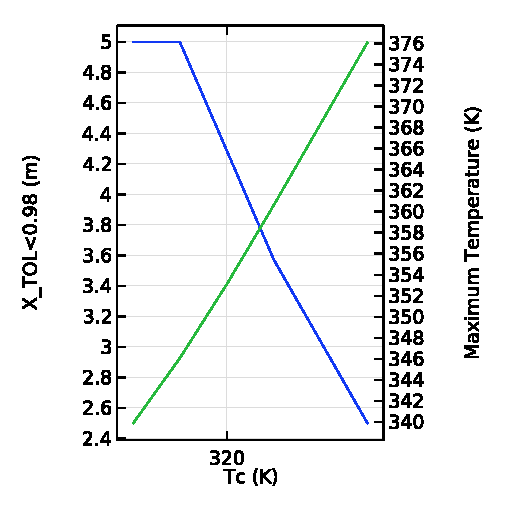
\includegraphics[width=0.49\linewidth]{figures/S4-CW-X-T.eps}
    \caption{Effect of CW temperature on distance required to reach 98\% conversion (blue) and max T (green)}
    \label{fig:comsol-S4-CW-X-T}
\end{figure}
